\subsection{Exemplo de execução}
\label{sec:exemplo_execucao}

Para ilustrar o movimento \textit{move end-effector to target position}, apresenta-se uma execução completa no CoppeliaSim, na qual o manipulador apanha um cubo vermelho, detetado pela câmara na posição $(X, Y, Z) = (0{,}225;\ 0{,}149;\ 0{,}010)$~m do referencial do mundo, e o leva até ao alvo verde. As posições são convertidas para o referencial da base através da função \texttt{world\_to\_base}, e a função \texttt{plan\_vertical} escolhe, antes de o braço se mover, a inclinação da garra para cada descida.

O cubo encontra-se a 30~cm do eixo da base, fora da zona em que a garra pode descer na vertical (Figura~\ref{fig:mapa_alvos}), pelo que é apanhado com uma inclinação de $70^\circ$. O alvo verde, mais próximo da base, permite pousar o cubo com uma inclinação de $95^\circ$.

A sequência, apresentada na Figura~\ref{fig:execucao}, é a seguinte:
\begin{enumerate}
    \item o manipulador parte da pose inicial (Figura~\ref{fig:execucao}a);
    \item a função \texttt{move\_joints} leva a garra até à posição de aproximação, por cima do cubo, e a função \texttt{move\_linear} desce até ele, que é agarrado (Figura~\ref{fig:execucao}b);
    \item a garra sobe, desloca-se até por cima do alvo verde e desce até à posição de pouso, onde o cubo é largado (Figura~\ref{fig:execucao}c);
    \item a garra sobe e a função \texttt{go\_home} leva o manipulador de volta à pose inicial (Figura~\ref{fig:execucao}d).
\end{enumerate}

\begin{figure}[H]
  \centering
  \begin{minipage}[b]{0.48\textwidth}
    \centering
    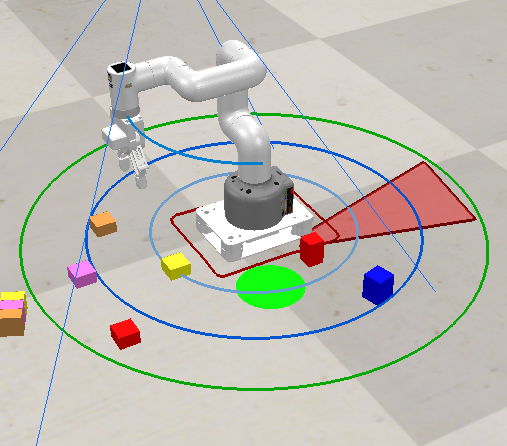
\includegraphics[width=\linewidth]{img/exec_1.png}\\[2pt]
    {\footnotesize (a) pose inicial}
  \end{minipage}\hfill
  \begin{minipage}[b]{0.48\textwidth}
    \centering
    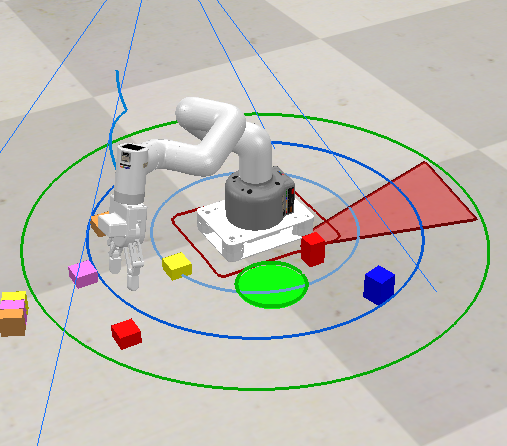
\includegraphics[width=\linewidth]{img/exec_2.png}\\[2pt]
    {\footnotesize (b) aproximação, por cima do cubo}
  \end{minipage}

  \vspace{6pt}
  \begin{minipage}[b]{0.48\textwidth}
    \centering
    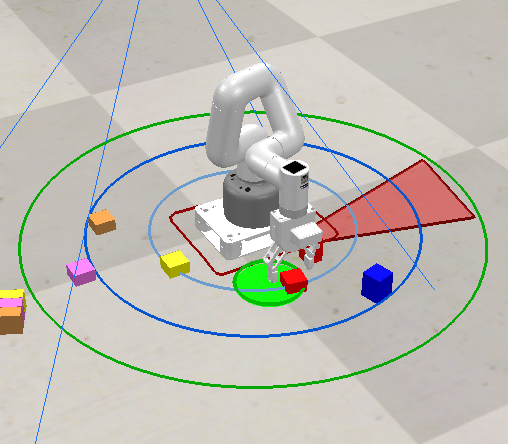
\includegraphics[width=\linewidth]{img/exec_3.png}\\[2pt]
    {\footnotesize (c) no alvo, a pousar o cubo}
  \end{minipage}\hfill
  \begin{minipage}[b]{0.48\textwidth}
    \centering
    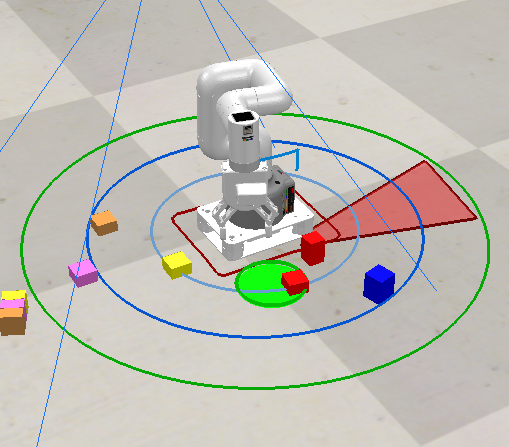
\includegraphics[width=\linewidth]{img/exec_4.png}\\[2pt]
    {\footnotesize (d) regresso à pose inicial}
  \end{minipage}
  \caption{Execução no CoppeliaSim: o cubo vermelho é levado até ao alvo verde. Na mesa estão desenhadas as zonas de alcance da Figura~\ref{fig:mapa_alvos}.}
  \label{fig:execucao}
\end{figure}

O Código~\ref{lst:execucao} apresenta a informação escrita pelo programa durante esta execução.

\begin{lstlisting}[basicstyle=\ttfamily\scriptsize, frame=single, breaklines=true,
                   caption={Saída do programa durante a execução da Figura~\ref{fig:execucao}.},
                   label={lst:execucao}]
--- tarefa 1 de 4 ---
pick_and_place: objeto no mundo [0.225 0.149 0.010], a 30 cm do eixo da base
pick_and_place: apanhar com a garra a 70 graus (J1 roda 38 graus), pousar a 95 graus (J1 roda 58 graus)
check_place: peça no sítio (red, 0.0 mm: não corrijo abaixo de 3 mm)
check_place: pilha deslocada 34.1 mm (green) -> [-0.021 0.177] em vez de [-0.000 0.150]
pick_and_place: concluído
Simulation time: 73.20 [s]
\end{lstlisting}

Antes de pousar o cubo, a câmara confirma a posição do destino. Nesta execução, o alvo verde foi detetado a 34,1~mm da posição esperada, e o ponto de pouso foi corrigido para a nova posição antes da descida. O movimento completo demorou 73,2~s de tempo de simulação. Os erros de posicionamento em diferentes posições alvo são apresentados na Tabela~\ref{tab:demo_sim}.